\chapter{DevOps}
\label{chapter:mant}

Una vez hemos llegado a esta parte del documento ya hemos realizado el análisis completo de los datos y hemos dejado el modelo en un entorno productivo clasificando llamadas en \textit{real-time}; sin embargo sería muy atrevido dar el proyecto por finalizado.

Probablemente surgirán nuevos datos, dispondremos de nuevas etiquetas, nuestro \textit{software} se degradará, crearemos nuevos y mejores modelos con ideas más o menos brillantes, etc. Este universo cambiante provocará a que se modificarán y/o se crearán nuevos \textit{software} y modelos con bastante frecuencia que será necesario llevar de nuevo a producción.  

Este capítulo tiene objetivo definir los mecanismos y la metodología que hemos establecido para poder reaccionar con gran agilidad ante el cambio, algo esencial hoy en día. En la sección \ref{section:mant:devops} haremos una introducción a la metodología DevOps que acuñaremos en nuestro proyecto, posteriormente pondremos foco en algunos aspectos importantes: La degradación del modelo (sección \ref{section:mant:efi}) y la integración y el despliegue continuos (sección \ref{section:mant:cicd}).


\section{Introducción DevOps}
\label{section:mant:devops}


\begin{figure}[!ht]
	\centering
	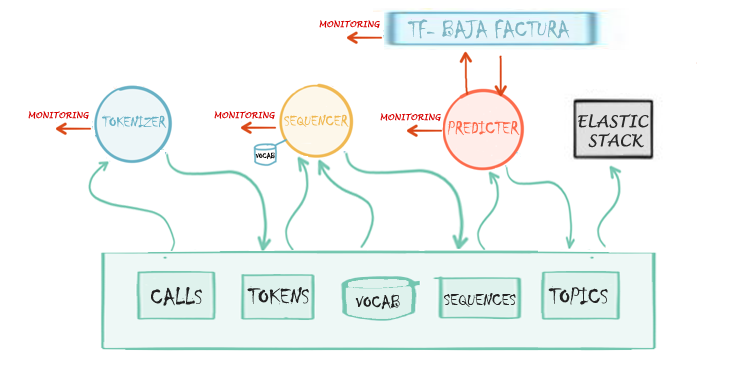
\includegraphics[width=1\textwidth]{images/exp/micro-arch-v3}
	\caption{Arquitectura microservicios}
	\label{fig:micro-arch}
\end{figure}

\section{Degradación del modelo}
\label{section:mant:efi}
Aunque el \textit{software} desarrollado también es propenso de degradarse con el paso del tiempo, si hay algo que tenemos seguro que se va a degradar en este universo cambiante es el modelo. Nuestro modelo se alimenta con las transcripciones de los clientes que están basadas en el servicio que ofrecemos en cada momento, en las inquietudes de nuestros clientes y otros muchos factores externos que pueden influir en la temática de las conversaciones que recibimos.

La certeza en la degradación de nuestro modelo hace que tengamos monitorizar constantemente el rendimiento del mismo, en el caso del modelo supervisado que hemos llevado a producción nos lleva a seguir testeándolo constantemente introduciendo en el flujo llamadas de control etiquetadas para medir su eficiencia.  




\section{Integración y despliegue continuos}
\label{section:mant:cicd}